\documentclass[12pt]{article}
\usepackage{amsmath}
\usepackage{amssymb}
\usepackage{amsthm}
\usepackage{color}
\usepackage{graphicx}
\usepackage{natbib}
\usepackage{xspace}
\linespread{1.7}

\newcommand{\sdgphi}{\ensuremath{\sigma_{g\phi}}\xspace}
\newcommand{\sdphi}{\ensuremath{\sigma_{\phi}}\xspace}
\newcommand{\sdmu}{\ensuremath{\sigma_{\mu}}\xspace}
\newcommand{\dnorm}{\ensuremath{\mathbf{\Phi}}}{\xspace}

\begin{document}
\setlength{\parindent}{0cm}
List of figures and explanations for them, including the captions for the figures, and how to reproduce them.\\
\begin{figure}[h]
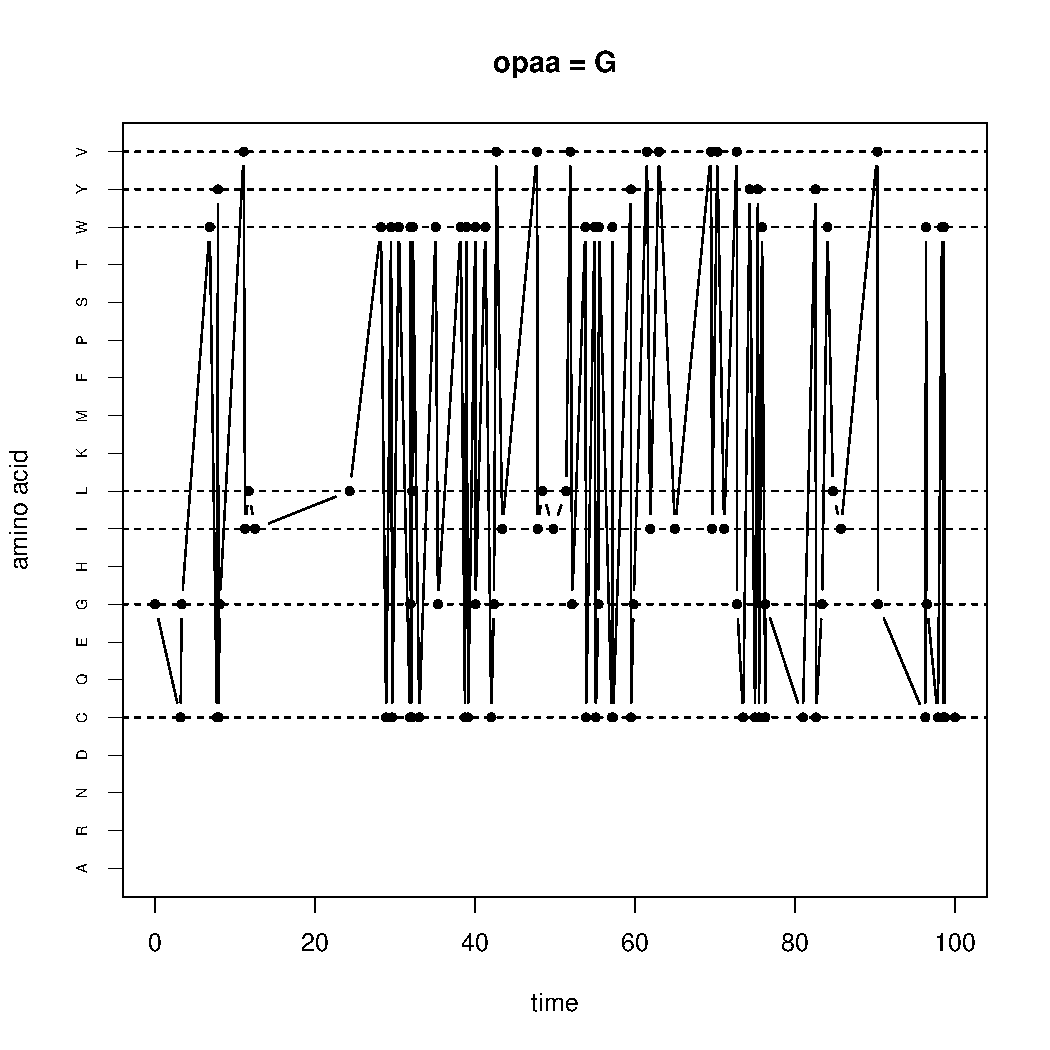
\includegraphics[width=\textwidth]{evopath_opaa8.pdf}
\caption{A long evolutionary path when the optimal amino acid is (8th) G. With 84 substitutions in the path, only 7 states are visited. Parameter values are: $g\phi = 2.005282$, $\beta = 0.1938331$, $\gamma = 0.0003889893$, $Q = {1.129544, 3.032109, 1.381705, 1.751379, 3.799967, 1.000000}$}
\label{fig:evopath}
\end{figure}

To reproduce Figure~\ref{fig:evopath}, use the function {\it simulation} to do the simulation and then plot the path. The number of amino acids in the simulated protein can be longer than 1. 

%%%%%%%%%%%%%%%%%%%%%%%%%%%%%
\begin{figure}[h]
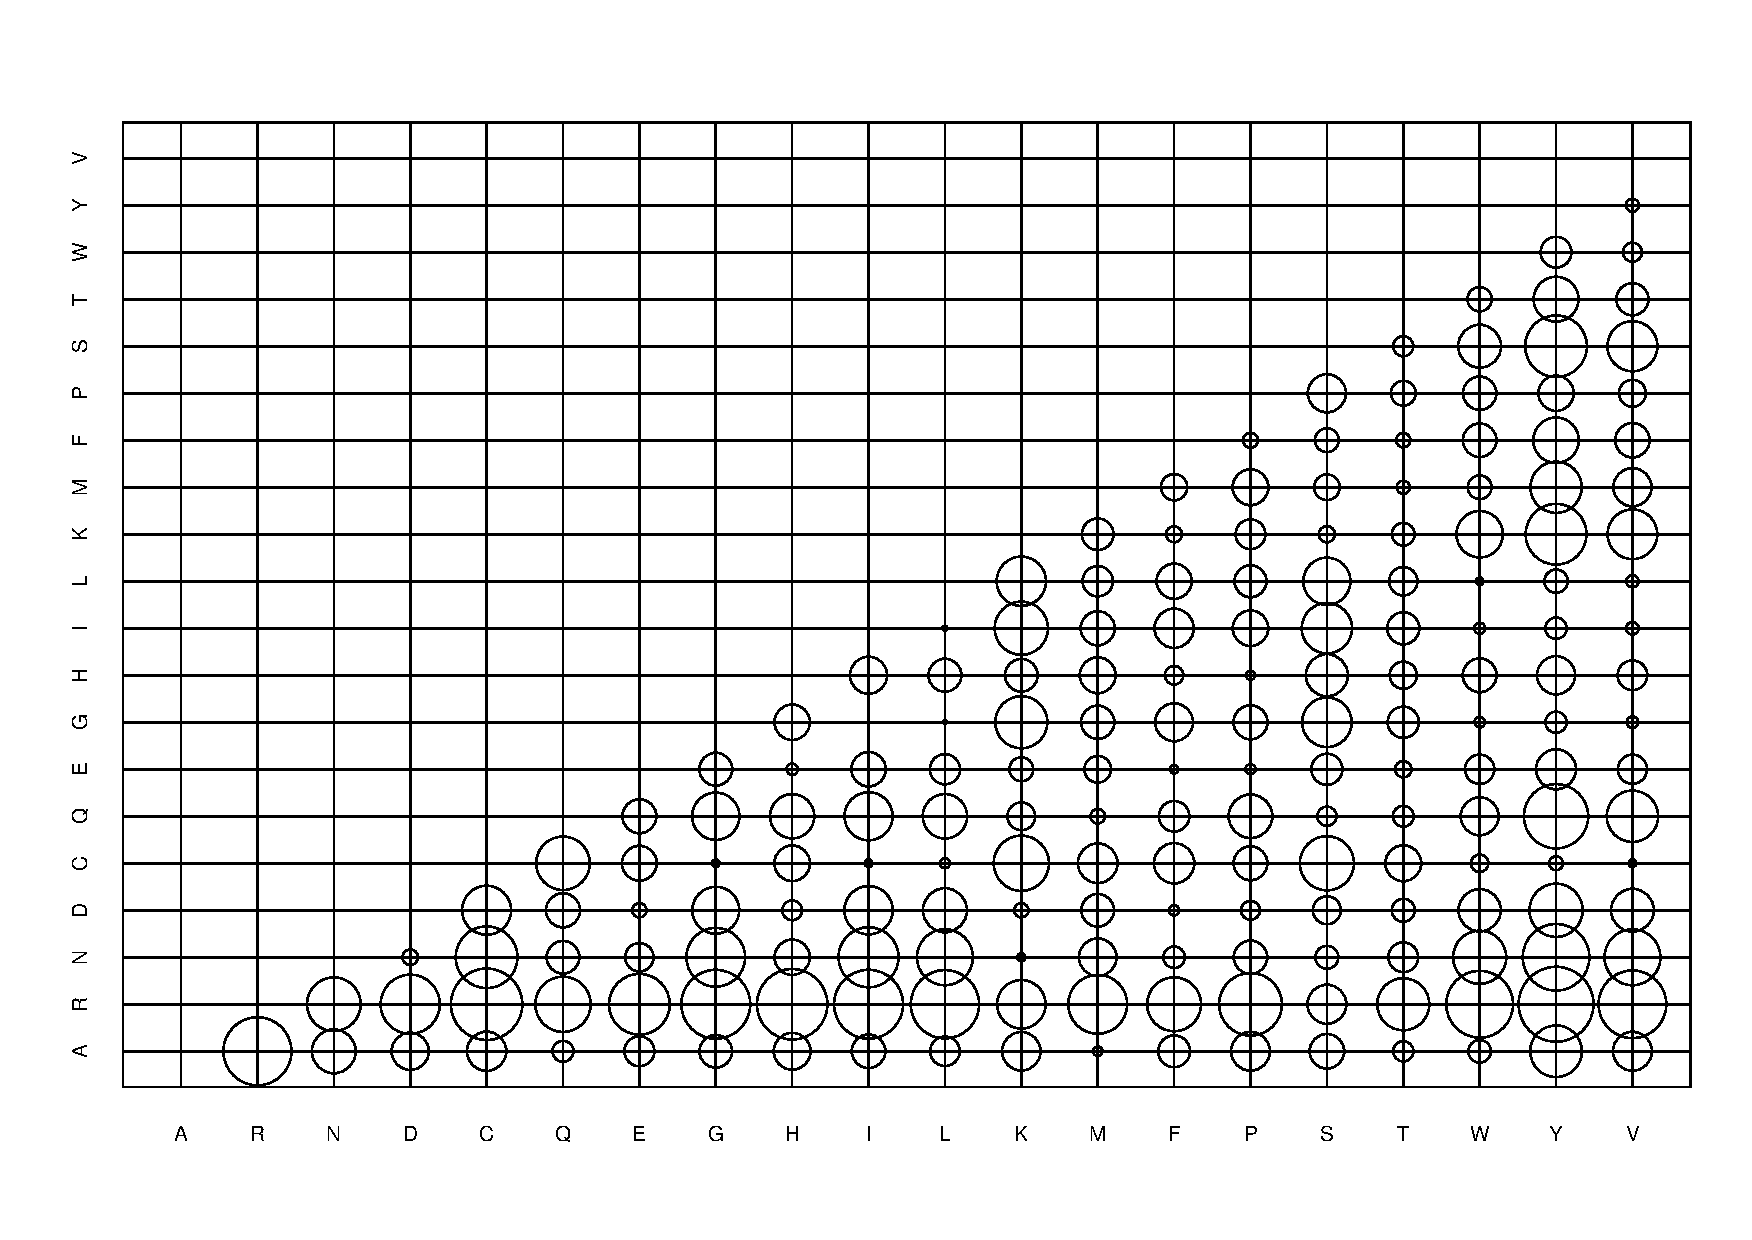
\includegraphics[width=\textwidth]{GranthamMatrix.pdf}
\caption{Bubble plot of the Grantham Distance matrix with Grantham's weights. Only half of the matrix is plotted since it's symmetric.}
\label{fig:GranthamDis}
\end{figure}
Plot function for this Figure~\ref{fig:GranthamDis} is {\it matrix.bubble}.

%%%%%%%%%%%%%%%%%%%%%%%%%%%%%
\begin{figure}[h]
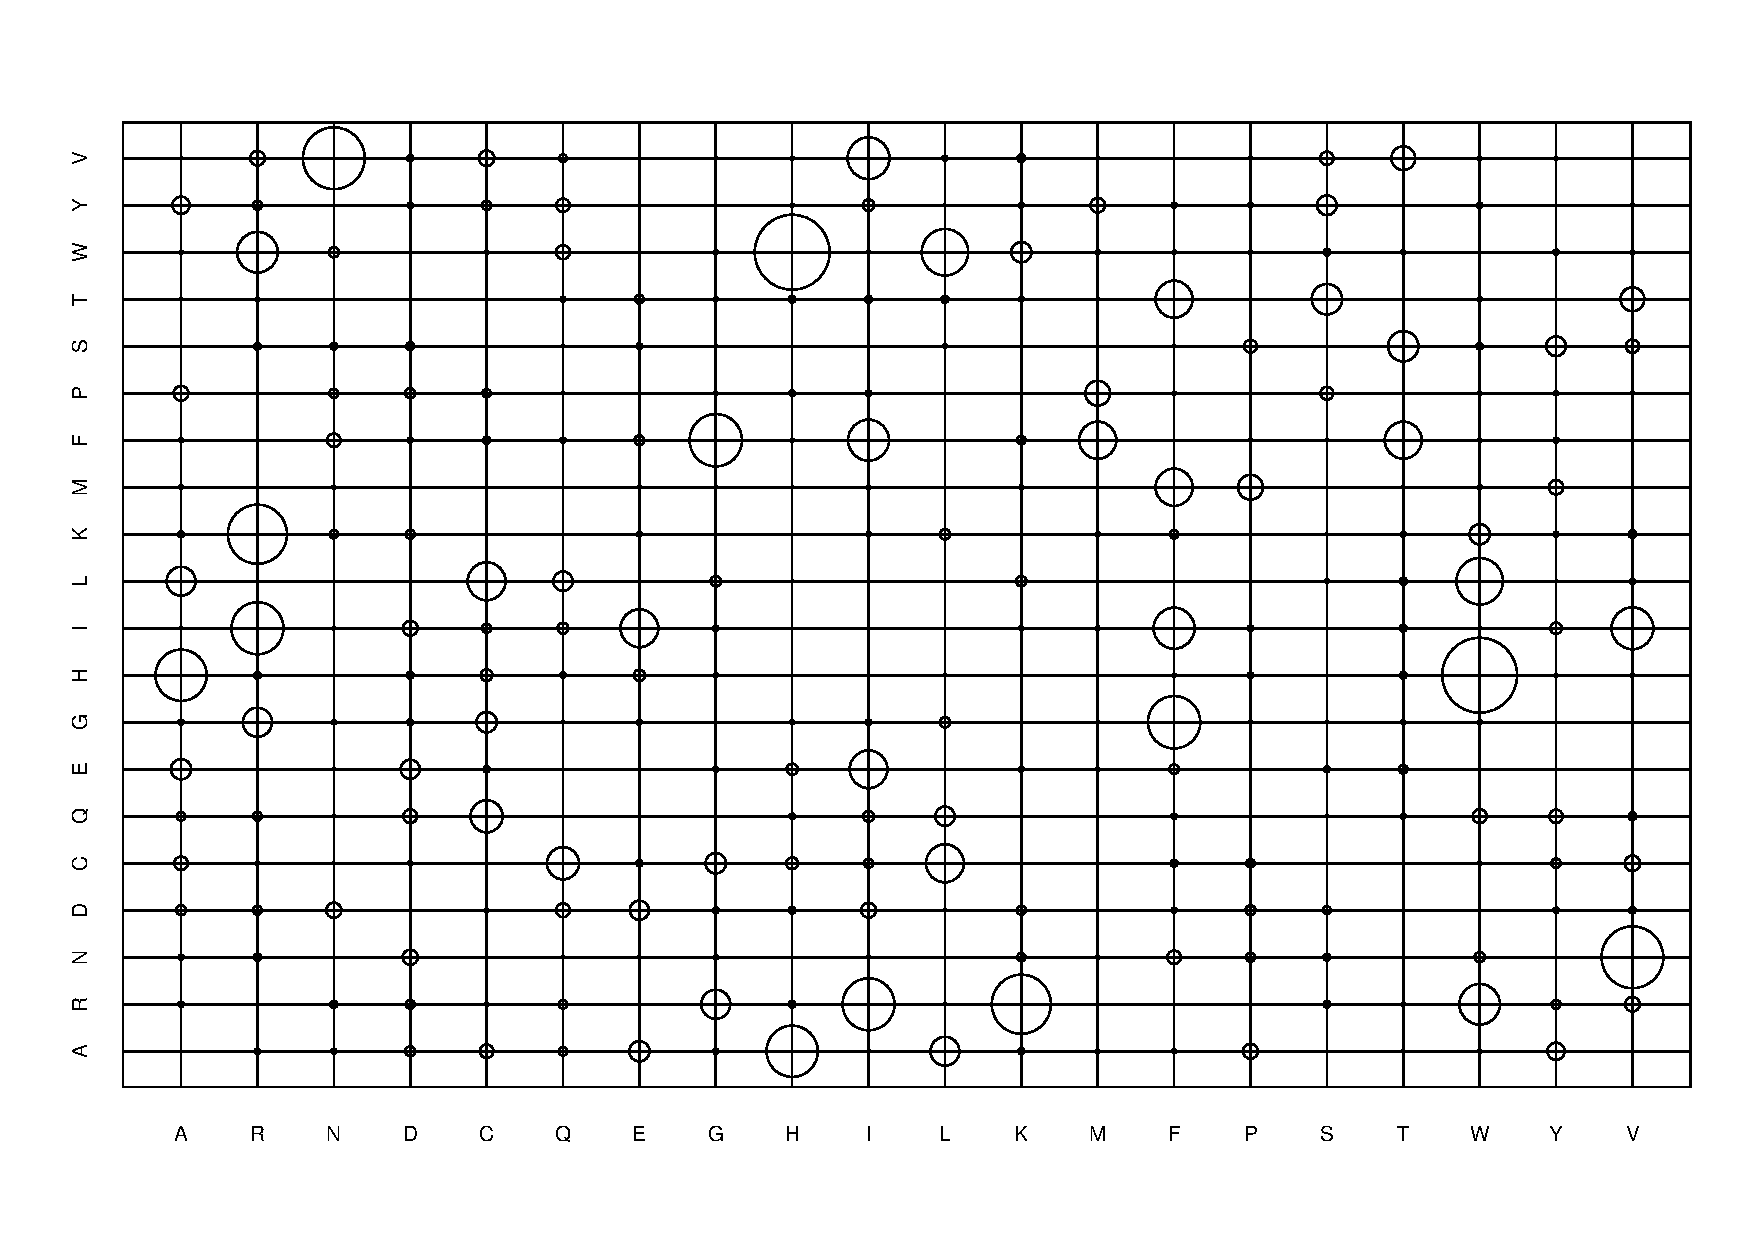
\includegraphics[width=\textwidth]{WAG_submat.pdf}
\caption{Bubble plot of the substitution rates matrix under WAG model. Only half of the matrix is plotted since it's symmetric.}
\label{fig:WAGmat}
\end{figure}

%%%%%%%%%%%%%%%%%%%%%%%%%%%%%
\begin{figure}[h]
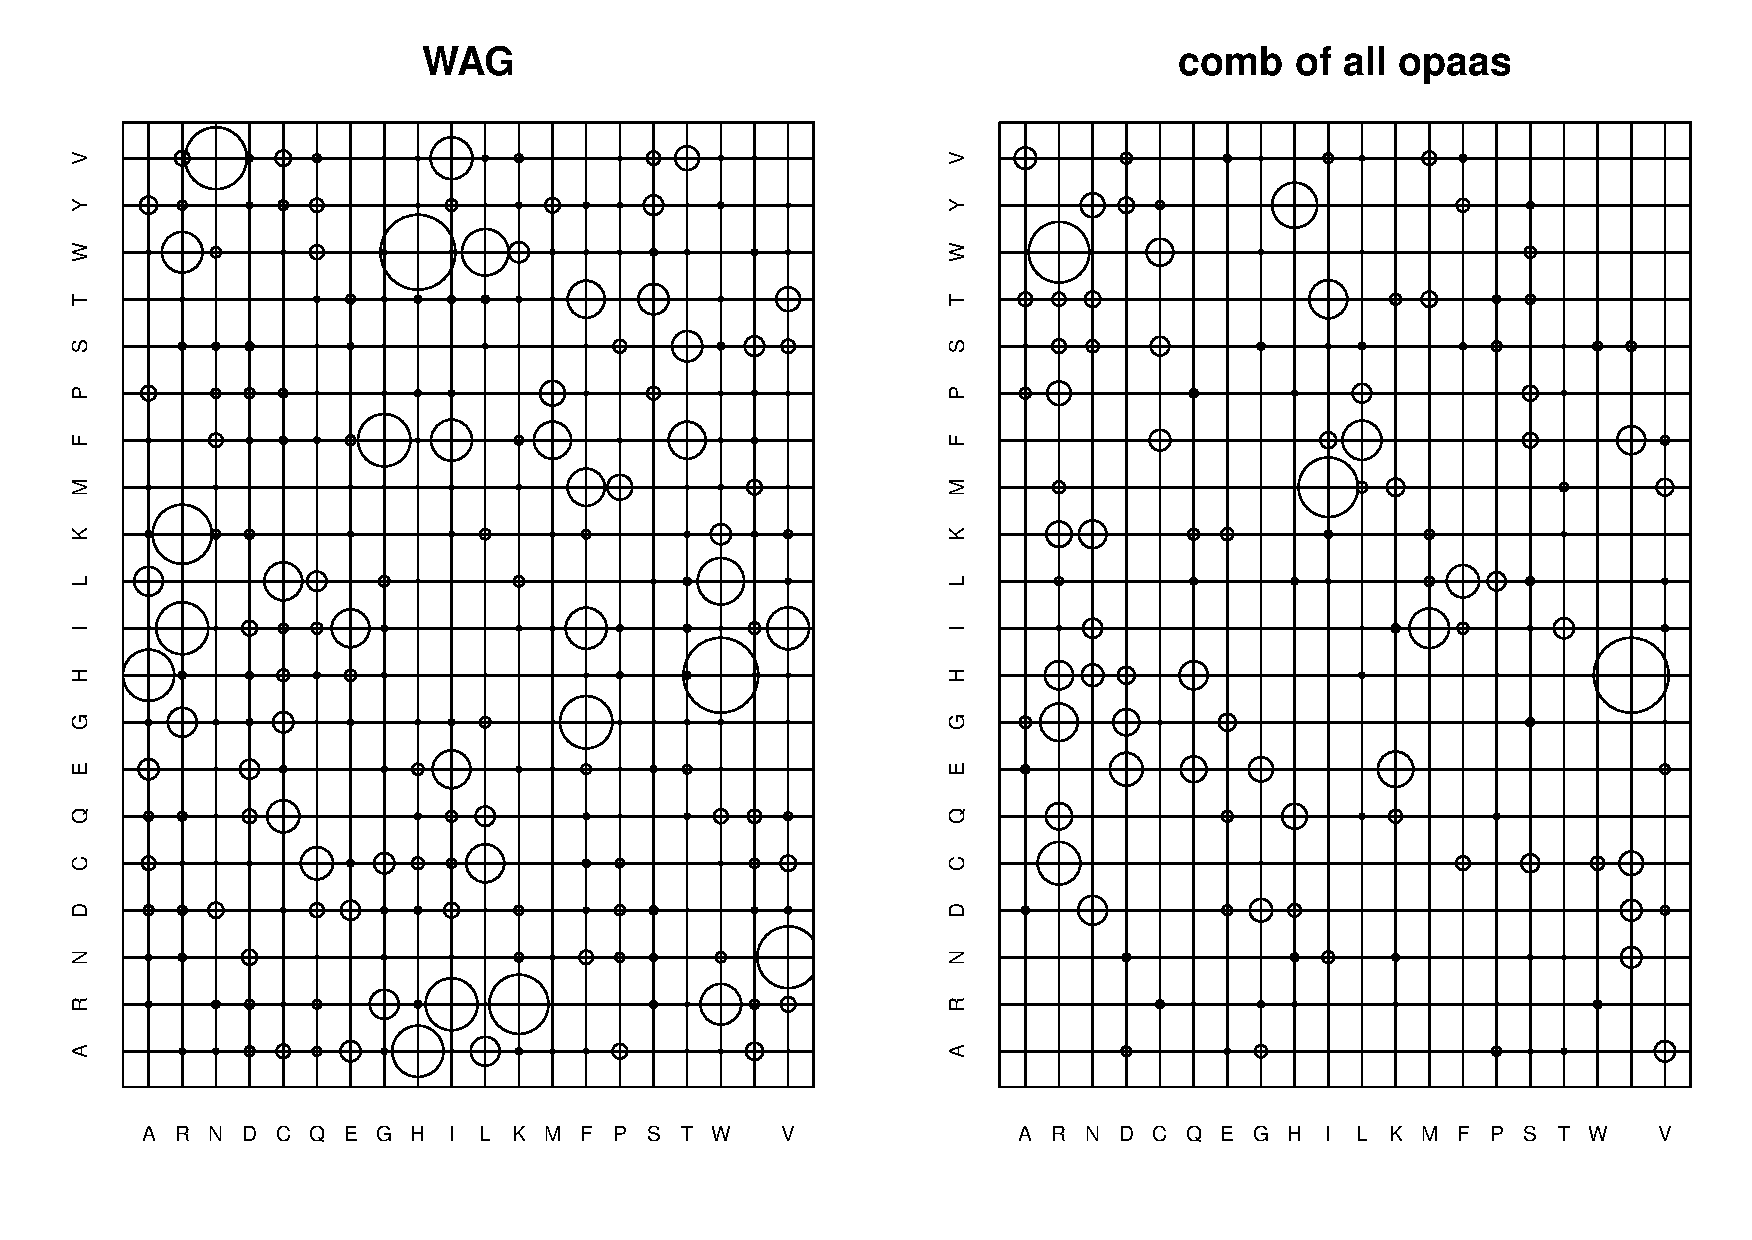
\includegraphics[width=\textwidth]{WAGvsMash.pdf}
\caption{Substitution rate matrix under WAG model and a mash of substitution rate matrices for all amino acids being optimal.}
\label{fig:WAG-Mash}
\end{figure}

Like Figure~\ref{fig:WAG-Mash}, plots of all substitution rate matrices for each amino acid being optimal are in {\bf submit\_all\_opaa.pdf}.
%%%%%%%%%%%%%%%%%%%%%%%%%%%%%
\begin{figure}[h]
\centering
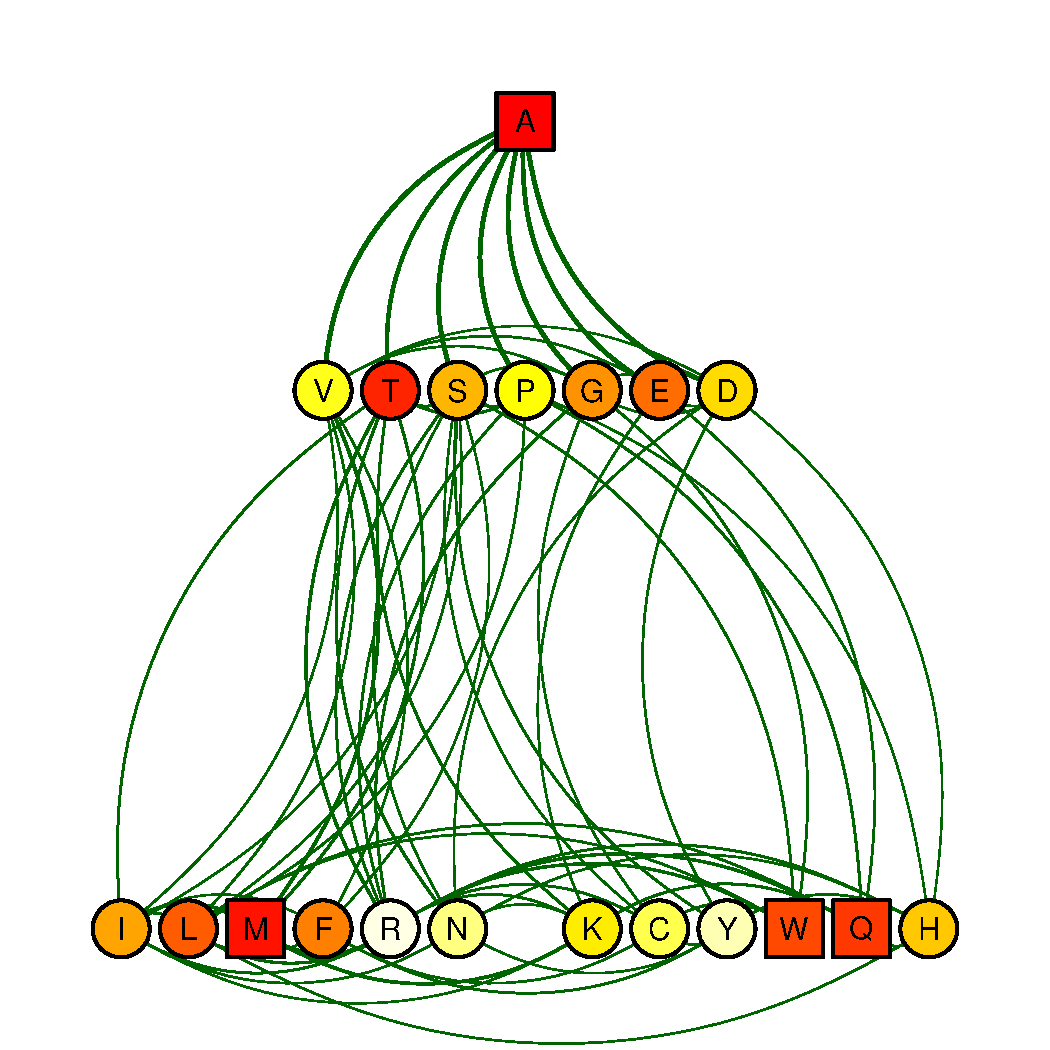
\includegraphics[page=1,width=0.6\textwidth]{network_A.pdf}
\includegraphics[page=2,width=0.6\textwidth]{network_A.pdf}
\caption{Another visualization of the substitution matrix. Squared nodes are local optima, the top one shows the neighboring amino acids more clearly.}
\label{fig:network}
\end{figure}

All the network figures like Figure~\ref{fig:network} are in {\bf network\_plots.pdf} and {\bf network\_plots\_nolevel.pdf}. They are produced by the functions {\it fgraph} and {\it fgraph1}.

%%%%%%%%%%%%%%%%%%%%%%%%%%%%%
\begin{figure}[h]
\centering
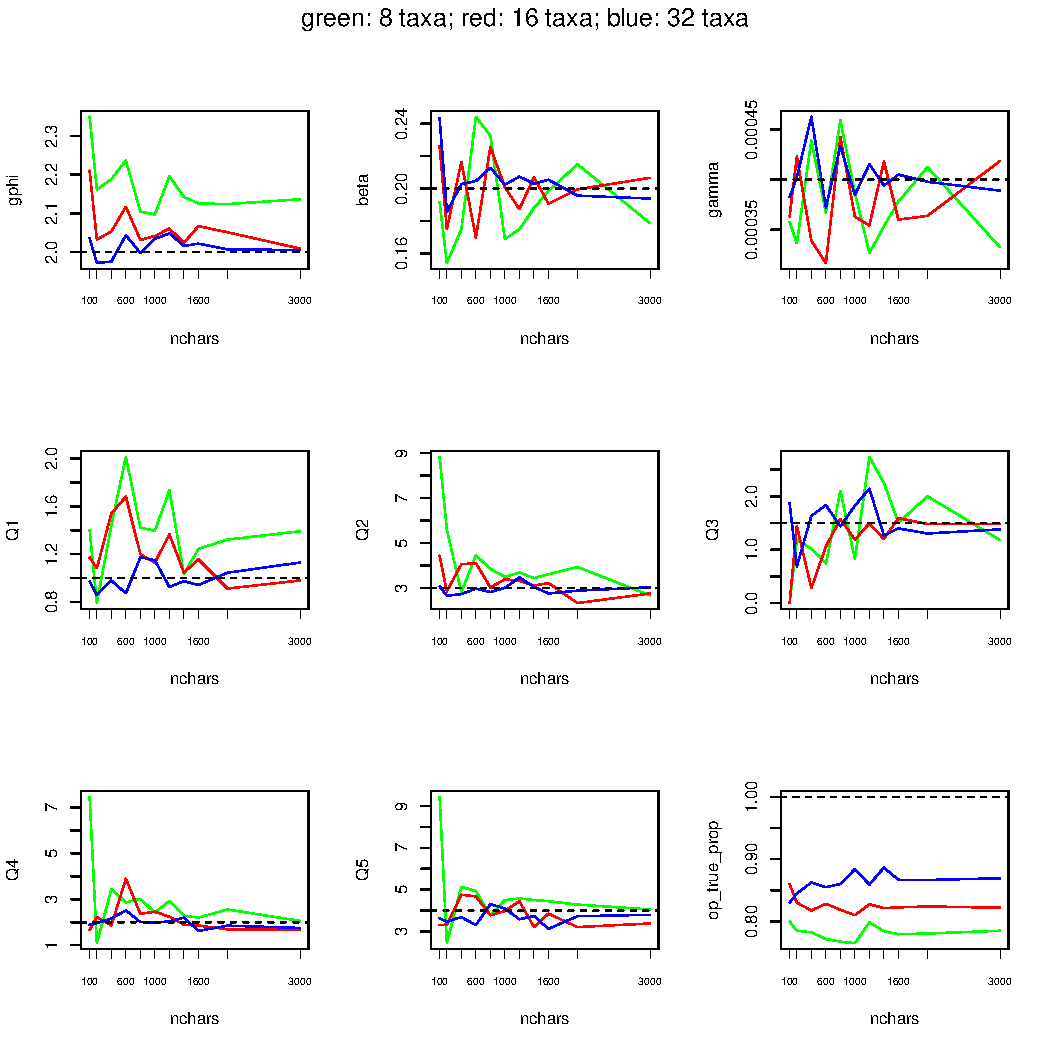
\includegraphics[width=\textwidth]{para_est_simfromsim.pdf}
\caption{Parameter estimation from simulated data. The last panel is the proportion of the correctly inferred optimal amino acids of all sites. This shows that as the number of taxa or characters increases the parameter estimates are more accurate. }
\label{fig:paraEst}
\end{figure}

Figure~\ref{fig:paraEst} is plotted by {\bf gatherdata.R}.

%%%%%%%%%%%%%%%%%%%%%%%%%%%%%
\begin{figure}[h]
\centering
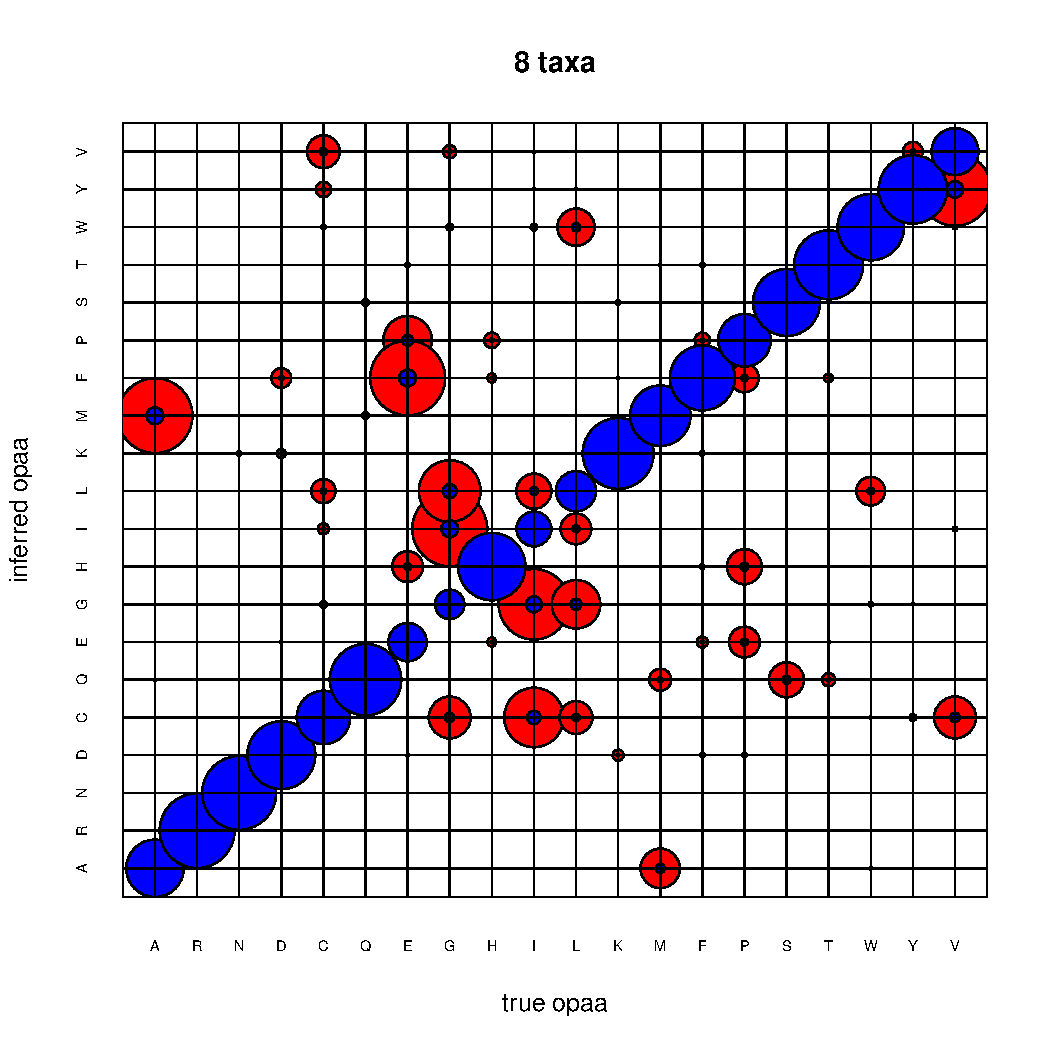
\includegraphics[page=1,width=\textwidth]{opaa_estimation_combined.pdf}
\caption{Inference of optimal amino acids from simulated data. Red ones are the magnified version of the incorrectly inferred optimal amino acids.}
\label{fig:opaaEst}
\end{figure}

Figure~\ref{fig:opaaEst} is plotted by {\bf test.R}, and plots for 16 and 32 taxa are in \\{\bf opaa\_estimation\_combined.pdf}.

%%%%%%%%%%%%%%%%%%%%%%%%%%%%%
\begin{figure}[h]
\centering
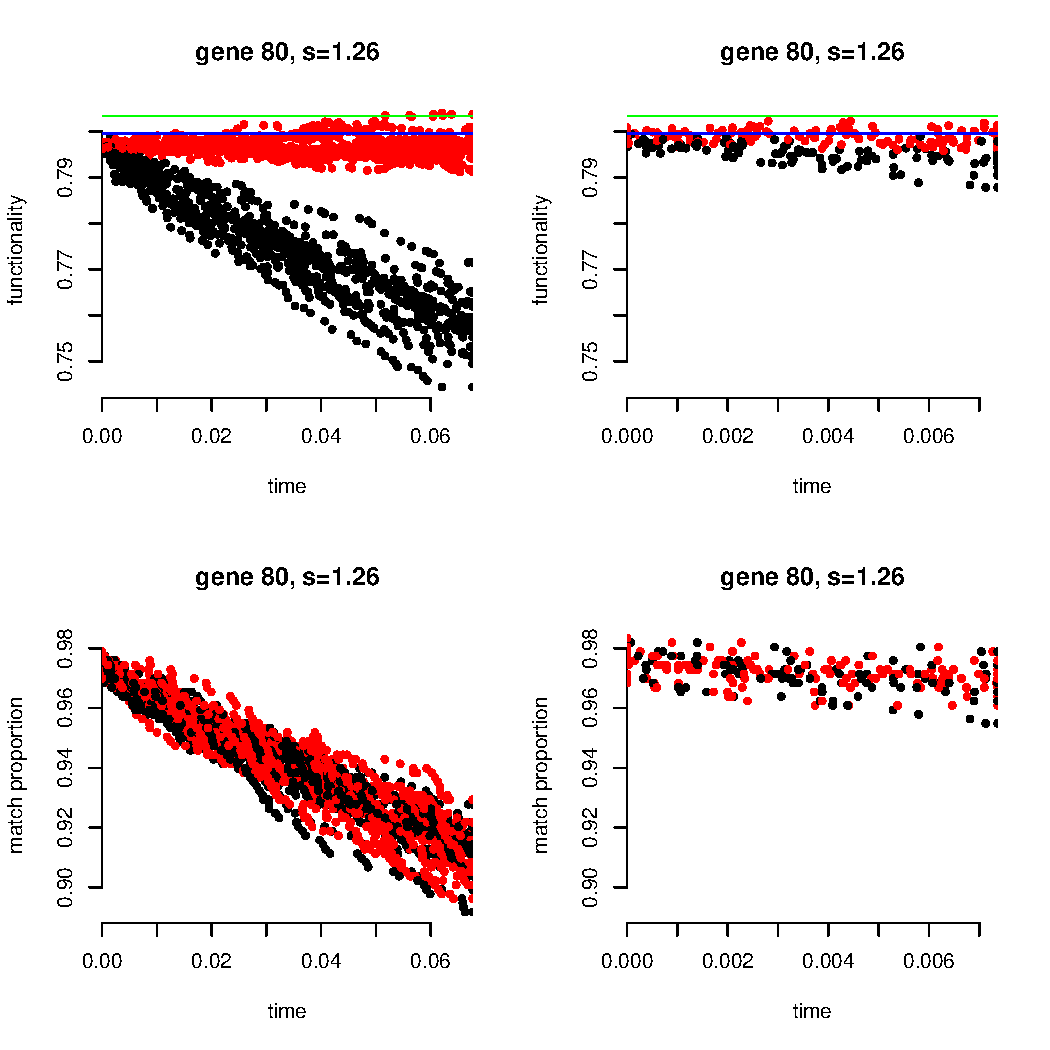
\includegraphics[width=0.8\textwidth]{gene80_adequacy.pdf}
\caption{Model adequacy illustration. One external branch is broken off the tree for yeast data, and the grafted back, under both best empirical model for the gene and the new model. Top panels are the functionalities of protein sequence along the evolutionary path, and the bottom panels are the matching proportion to the observed data. Red is simulation under new model, black is simulation under empirical model. Blue line the observed functionality, green line is the equilibrium functionality.}
\label{fig:adequacy}
\end{figure}

All figures like Figure~\ref{fig:adequacy} are in this directory: \\ {\bf $\sim$/BackupProEvo/Newton/yeast/adequacy}
%%%%%%%%%%%%%%%%%%%%%%%%%%%%%
\begin{figure}[h]
\centering
\includegraphics[page=2,width=\textwidth]{gene80_sim.pdf}
\caption{Same gene (80th), functionality of simulated sequence under the estimated parameter values, comparing to the observed sequences.}
\label{fig:sim-func}
\end{figure}

\begin{figure}[h]
\centering
\includegraphics[page=3,width=\textwidth]{gene80_sim.pdf}
\caption{Same gene (80th), similarity of simulated sequence under the estimated parameter values, to the observed sequences.}
\label{fig:sim-similarity}
\end{figure}

All figures like Figure~\ref{fig:sim-func} and Figure~\ref{fig:sim-similarity} are in this directory: \\ {\bf $\sim$/BackupProEvo/Newton/yeast/rootEqm}.
\end{document}


